\section{Experimental Results}
\label{sec:results}

This section reports and discusses results for the four research questions in Section~\ref{sec:rqs}. LoRA per task serves as the upper-bound reference in every comparison because it uses the true task label at inference; every other method, including GMM-Router, must infer the task from the input alone.

\subsection{RQ1: Performance on the CodeTask benchmark}
\label{sec:codetask_results}

Table~\ref{tab:codetask_qwen} reports the final per-task and average scores on the CodeTask benchmark after the model has learned the full eight-task sequence.

\begin{table}[t]
\centering
\caption{Final results (\%) on the CodeTask benchmark (Qwen2.5-Coder-1.5B, $\tau=2.0$). LoRA per task is the upper bound (task identity known at inference).}
\label{tab:codetask_qwen}
\scriptsize
\resizebox{\linewidth}{!}{%
\begin{tabular}{lccccccccc}
\toprule
Method & CONCODE & CodeTrans & CodeSearchNet & BFP & KodCode & RunBugRun & TheVault & CoST & Avg. \\
\midrule
LoRA per task & 36.56 & 77.55 & 16.00 & 80.15 & 54.20 & 66.11 & 26.48 & 76.17 & 54.15 \\
\midrule
EWC & 8.54 & 17.79 & 2.73 & 41.48 & 8.74 & 37.56 & 18.28 & 70.40 & 25.69 \\
L2P & 5.62 & 23.32 & 2.60 & 35.09 & 6.36 & 24.98 & 2.21 & 34.34 & 16.82 \\
ProgPrompt & 11.83 & 34.34 & 1.88 & 35.90 & 15.93 & 18.23 & 1.87 & 68.90 & 23.61 \\
SeqLoRA & 14.04 & 37.96 & 1.99 & 62.64 & 20.02 & 64.10 & 2.53 & 75.92 & 34.90 \\
O-LoRA & 10.84 & 36.09 & 13.80 & 77.24 & 41.77 & 65.89 & 21.21 & 75.34 & 42.77 \\
Online-CL-LLM & 22.52 & 47.97 & 14.65 & 68.57 & 25.22 & 64.83 & 15.24 & 71.87 & 41.36 \\
TreeLoRA & 14.85 & 34.58 & 2.12 & 44.24 & 17.27 & 78.18 & 2.16 & 83.20 & 34.58 \\
\midrule
\textbf{GMM-Router} & 35.06 & 73.48 & 14.85 & 79.95 & 51.75 & 63.12 & 18.51 & 76.26 & 51.62 \\
\bottomrule
\end{tabular}%
}
\end{table}

GMM-Router reaches the highest average (51.62\%) among all task-agnostic methods, ahead of O-LoRA (42.77\%) and Online-CL-LLM (41.36\%) by a wide margin and close to the LoRA per task upper bound (54.15\%). The advantage stems from three design choices acting together (Section~\ref{sec:methodology}): task-isolated LoRA adapters that prevent gradient interference, a stable routing space from the fixed orthonormal projection $\mathbf{P}$ applied to frozen backbone features, and hard routing that assigns each input deterministically to its best-matching expert via GMM log-posteriors under a uniform class prior.

GMM-Router is strongest on BFP (79.95\%), CoST (76.26\%), and CodeTrans (73.48\%), all close to or matching the upper bound, indicating that dedicated experts with stable routing suffice for these structured tasks. It is weaker on TheVault (18.51\%) and CodeSearchNet (14.85\%), both code-to-text generation tasks whose broad, less distinctive input distributions are harder to separate by density estimation alone. Among the baselines, O-LoRA and Online-CL-LLM are strongest, reflecting the benefit of orthogonal subspaces and feature-based block selection, respectively; SeqLoRA (34.90\%) and TreeLoRA (34.58\%) trail, and EWC (25.69\%), ProgPrompt (23.61\%), and L2P (16.82\%) are substantially weaker, indicating that shallow regularization or limited prompt capacity is insufficient for this diverse benchmark.

\subsection{RQ2: Performance on the executable benchmark}
\label{sec:exec_results}

Table~\ref{tab:exec_avg} reports average Pass@1 and Pass@5 on the executable benchmark.

\begin{table}[t]
\centering
\caption{Average Pass@1 and Pass@5 (\%) on the executable benchmark. LoRA per task is the upper bound (task identity known, without iterative refinement).}
\label{tab:exec_avg}
\small
\begin{tabular}{lcc}
\toprule
Method & Avg.\ Pass@1 (\%) & Avg.\ Pass@5 (\%) \\
\midrule
LoRA per task & 33.46 & 42.19 \\
\midrule
EWC & 0.09 & 0.22 \\
L2P & 8.03 & 11.75 \\
ProgPrompt & 28.01 & 40.00 \\
SeqLoRA & 37.51 & 45.67 \\
O-LoRA & 33.71 & 42.09 \\
Online-CL-LLM & 33.50 & 41.95 \\
TreeLoRA & 36.84 & 46.37 \\
\midrule
\textbf{GMM-Router} & 34.40 & 47.75 \\
\bottomrule
\end{tabular}
\end{table}

GMM-Router reaches 34.40\% Pass@1 and 47.75\% Pass@5. On Pass@1, SeqLoRA (37.51\%) and TreeLoRA (36.84\%) lead, benefiting from cross-task transfer that a shared or hierarchically shared adaptation space provides on this benchmark, which is homogeneous in task format across nine syntactically related languages. On Pass@5, GMM-Router leads all methods (47.75\%), ahead of TreeLoRA (46.37\%) and SeqLoRA (45.67\%), indicating that soft routing produces a more diverse candidate set that collectively covers more of the problem space. GMM-Router's Pass@1 (34.40\%) slightly exceeds the non-iterative LoRA per task upper bound (33.46\%); this improvement is attributable to the iterative refinement pipeline recovering samples that fail every Round-1 candidate (RQ4, Section~\ref{sec:refinement}). GMM-Router also outperforms O-LoRA (33.71\%/42.09\%) and Online-CL-LLM (33.50\%/41.95\%), consistent with per-task GMM density estimation in a stable, fixed-projection routing space providing a more reliable task-distribution model than orthogonality constraints or feature-distribution matching alone. EWC (0.09\% Pass@1) and L2P (8.03\%) perform poorly, indicating that regularization and shallow prompt selection are insufficient for generating functionally correct multilingual code. The gap to SeqLoRA ($-3.11$pp Pass@1) reflects a trade-off examined further in Section~\ref{sec:crossbench}: SeqLoRA's shared adaptation accumulates cross-language knowledge on this homogeneous benchmark but forgets severely on the diverse CodeTask sequence (34.90\% vs.\ GMM-Router's 51.62\%, Table~\ref{tab:codetask_qwen}).

\subsubsection{Per-language analysis}
\label{sec:perlang}

Tables~\ref{tab:exec_p1} and~\ref{tab:exec_p5} report Pass@1 and Pass@5 for each programming language.

\begin{table}[t]
\centering
\caption{Per-language Pass@1 (\%) on the executable benchmark ($\tau=1.0$).}
\label{tab:exec_p1}
\scriptsize
\resizebox{\linewidth}{!}{%
\begin{tabular}{lccccccccc}
\toprule
Method & Py & C++ & Swift & Rust & C\# & Java & PHP & TS & Shell \\
\midrule
LoRA per task & 43.59 & 6.80 & 59.20 & 22.64 & 1.20 & 18.87 & 36.40 & 93.20 & 19.20 \\
\midrule
EWC & 0.80 & 0.00 & 0.00 & 0.00 & 0.00 & 0.00 & 0.00 & 0.00 & 0.00 \\
L2P & 7.60 & 2.40 & 24.80 & 1.51 & 7.60 & 0.00 & 10.80 & 17.60 & 0.00 \\
ProgPrompt & 31.60 & 16.80 & 57.20 & 4.15 & 3.60 & 13.96 & 30.80 & 78.80 & 15.20 \\
SeqLoRA & 45.52 & 13.60 & 62.00 & 10.57 & 24.00 & 22.26 & 33.20 & 98.40 & 28.00 \\
O-LoRA & 42.40 & 11.20 & 63.60 & 11.70 & 0.80 & 18.49 & 36.80 & 95.20 & 23.20 \\
Online-CL-LLM & 42.80 & 21.20 & 42.00 & 8.30 & 25.20 & 20.75 & 30.80 & 90.80 & 19.60 \\
TreeLoRA & 42.80 & 4.40 & 63.60 & 32.08 & 14.80 & 21.51 & 34.40 & 95.60 & 22.40 \\
\midrule
\textbf{GMM-Router} & 38.40 & 5.60 & 66.40 & 19.62 & 2.80 & 23.40 & 34.80 & 92.80 & 25.80 \\
\bottomrule
\end{tabular}%
}
\end{table}

\begin{table}[t]
\centering
\caption{Per-language Pass@5 (\%) on the executable benchmark ($\tau=1.0$).}
\label{tab:exec_p5}
\scriptsize
\resizebox{\linewidth}{!}{%
\begin{tabular}{lccccccccc}
\toprule
Method & Py & C++ & Swift & Rust & C\# & Java & PHP & TS & Shell \\
\midrule
LoRA per task & 54.00 & 8.00 & 72.00 & 35.85 & 4.00 & 35.85 & 44.00 & 96.00 & 30.00 \\
\midrule
EWC & 2.00 & 0.00 & 0.00 & 0.00 & 0.00 & 0.00 & 0.00 & 0.00 & 0.00 \\
L2P & 14.00 & 4.00 & 30.00 & 3.77 & 14.00 & 0.00 & 14.00 & 26.00 & 0.00 \\
ProgPrompt & 46.00 & 32.00 & 76.00 & 9.43 & 8.00 & 24.53 & 48.00 & 92.00 & 24.00 \\
SeqLoRA & 54.00 & 18.00 & 74.00 & 20.75 & 36.00 & 28.30 & 38.00 & 100.00 & 42.00 \\
O-LoRA & 56.00 & 14.00 & 72.00 & 24.53 & 4.00 & 28.30 & 46.00 & 100.00 & 34.00 \\
Online-CL-LLM & 50.00 & 30.00 & 54.00 & 11.32 & 32.00 & 30.19 & 40.00 & 98.00 & 32.00 \\
TreeLoRA & 54.00 & 8.00 & 70.00 & 50.94 & 24.00 & 26.42 & 44.00 & 100.00 & 40.00 \\
\midrule
\textbf{GMM-Router} & 46.00 & 8.00 & 80.00 & 58.49 & 8.00 & 45.28 & 46.00 & 100.00 & 38.00 \\
\bottomrule
\end{tabular}%
}
\end{table}

GMM-Router leads all methods on Swift (66.40\% Pass@1, 80.00\% Pass@5) and on Java Pass@5 (45.28\%, well above the next best, SeqLoRA and O-LoRA at 28.30\%), suggesting soft routing produces diverse candidates that cover more of the Java problem space. TypeScript is the easiest language overall (92.80\% Pass@1, 100.00\% Pass@5 for GMM-Router and most strong baselines). Rust shows a diversity benefit from soft routing: GMM-Router's Pass@1 (19.62\%) trails TreeLoRA (32.08\%), yet its Pass@5 (58.49\%) exceeds TreeLoRA's (50.94\%). GMM-Router is weakest on C\# (2.80\%/8.00\%) and C++ (5.60\%/8.00\%); for C\#, methods with shared adaptation (SeqLoRA 24.00\%, Online-CL-LLM 25.20\%) perform substantially better, suggesting C\# benefits from cross-language transfer that per-task isolation cannot exploit. Python (38.40\% Pass@1) similarly falls behind SeqLoRA (45.52\%), consistent with a Python distribution close enough to other languages in this benchmark that shared adaptation provides a useful inductive bias.

\subsection{RQ3: Forgetting, transfer, and router assignment}
\label{sec:rq3}

\subsubsection{Router assignment analysis}
\label{sec:routing_analysis}

To understand which task distributions the GMM router can reliably separate, this subsection examines hard-routing confusion matrices ($\hat k=\operatorname{argmax}_k\alpha_k(x)$) at the final training step. On CodeTask, hard routing is the actual inference method; on the executable benchmark, Round-1 uses soft routing, so this analysis instead exposes where the argmax decision fails and motivates the traceback router used in Round-2.

\paragraph{CodeTask benchmark.} Figure~\ref{fig:confusion_codetask} shows the row-normalized confusion matrix after the full eight-task sequence (percentage of 1{,}000 test samples per true task hard-routed to each expert). The average accuracy is 90.6\%. BFP (98.3\%) and CoST (99.5\%) are routed almost perfectly because their distinctive input/output language combinations (Java bug patches; C++ source with C\# target) produce compact, well-separated GMM regions. The two weakest tasks are TheVault (82.6\%) and RunBugRun (86.4\%). Two systematic confusion patterns explain most off-diagonal mass: CodeTrans draws 10.8\% of TheVault and 5.8\% of CONCODE samples because all three tasks share Java or C\# as an input or output language; and CoST draws 9.0\% of RunBugRun, 8.6\% of CodeTrans, 6.7\% of KodCode, and 6.6\% of TheVault, reflecting both its C\# output overlapping with CodeTrans/TheVault and code-to-code transformation tasks sharing structural embedding patterns with translation. These confusions align with the performance gaps in Table~\ref{tab:codetask_qwen}: TheVault and RunBugRun show the largest gaps to their per-task upper bounds.

\begin{figure}[t]
\centering
\begin{tikzpicture}
  \foreach \r/\c/\v in {
    0/0/93.1, 0/1/5.8,  0/2/0.0,  0/3/0.0,  0/4/0.6,  0/5/0.0,  0/6/0.4,  0/7/0.1,
    1/0/0.0,  1/1/88.4, 1/2/0.0,  1/3/0.0,  1/4/0.0,  1/5/0.0,  1/6/3.0,  1/7/8.6,
    2/0/0.0,  2/1/1.2,  2/2/90.5, 2/3/0.0,  2/4/0.0,  2/5/8.2,  2/6/0.1,  2/7/0.0,
    3/0/0.0,  3/1/1.4,  3/2/0.0,  3/3/98.3, 3/4/0.0,  3/5/0.0,  3/6/0.0,  3/7/0.3,
    4/0/0.0,  4/1/1.5,  4/2/0.1,  4/3/0.0,  4/4/91.3, 4/5/0.1,  4/6/0.3,  4/7/6.7,
    5/0/0.0,  5/1/0.4,  5/2/4.1,  5/3/0.0,  5/4/0.0,  5/5/86.4, 5/6/0.1,  5/7/9.0,
    6/0/0.0,  6/1/10.8, 6/2/0.0,  6/3/0.0,  6/4/0.0,  6/5/0.0,  6/6/82.6, 6/7/6.6,
    7/0/0.0,  7/1/0.2,  7/2/0.0,  7/3/0.0,  7/4/0.2,  7/5/0.0,  7/6/0.0,  7/7/99.5%
  } {
    \fill[heatblue!\v!white]
      ({\c*\CTcs}, {-\r*\CTcs}) rectangle ({(\c+1)*\CTcs}, {-(\r+1)*\CTcs});
    \node[font=\tiny] at ({(\c+0.5)*\CTcs}, {-(\r+0.5)*\CTcs}) {\v};
  }
  \draw[gray!40, thin] (0,0) grid[xstep=\CTcs, ystep=\CTcs] ({8*\CTcs},{-8*\CTcs});
  \foreach \c/\lbl in {
    0/CONCODE, 1/CodeTrans, 2/CodeSearchNet, 3/BFP,
    4/KodCode, 5/RunBugRun, 6/TheVault, 7/CoST%
  } {
    \node[font=\tiny, anchor=north east, rotate=45]
      at ({(\c+0.5)*\CTcs}, {-8*\CTcs-0.05}) {\lbl};
  }
  \foreach \r/\lbl in {
    0/CONCODE, 1/CodeTrans, 2/CodeSearchNet, 3/BFP,
    4/KodCode, 5/RunBugRun, 6/TheVault, 7/CoST%
  } {
    \node[font=\tiny, anchor=east]
      at ({-0.08}, {-(\r+0.5)*\CTcs}) {\lbl};
  }
  \node[font=\scriptsize] at ({4*\CTcs}, {-9.0*\CTcs}) {Predicted Expert};
  \node[font=\scriptsize, rotate=90, anchor=center] at (-2.35, {-4*\CTcs}) {True Task};
\end{tikzpicture}
\caption{Hard-routing confusion matrix (\%) on the CodeTask benchmark at the final training step. Rows = true task; columns = assigned expert. Diagonal entries indicate correct routing; darker cells indicate higher routing weight.}
\label{fig:confusion_codetask}
\end{figure}

\paragraph{Executable benchmark.} Figure~\ref{fig:confusion_exec} shows the instruction router's confusion matrix after the full nine-language sequence. The average accuracy is only 15.8\%, sharply lower than on CodeTask. C++ dominates as a single attractor, drawing between 60\% (Python) and 100\% (C++ itself and TypeScript) of every language's samples; Python is the only exception, correctly routing 40.0\% of its own samples, while all other non-C++ languages score at most 2.0\%. This collapse occurs because the nine languages share deep syntactic overlap --- C-style braces, type keywords, similar control-flow constructs --- and because C++, trained second in the sequence, established broad coverage of the routing feature space before later languages' GMMs could carve out well-separated regions.

\begin{figure}[t]
\centering
\begin{tikzpicture}
  \foreach \r/\c/\v in {
    0/0/40.0, 0/1/60.0, 0/2/0.0, 0/3/0.0, 0/4/0.0, 0/5/0.0, 0/6/0.0, 0/7/0.0, 0/8/0.0,
    1/0/0.0,  1/1/100.0,1/2/0.0, 1/3/0.0, 1/4/0.0, 1/5/0.0, 1/6/0.0, 1/7/0.0, 1/8/0.0,
    2/0/0.0,  2/1/98.0, 2/2/2.0, 2/3/0.0, 2/4/0.0, 2/5/0.0, 2/6/0.0, 2/7/0.0, 2/8/0.0,
    3/0/11.3, 3/1/88.7, 3/2/0.0, 3/3/0.0, 3/4/0.0, 3/5/0.0, 3/6/0.0, 3/7/0.0, 3/8/0.0,
    4/0/4.0,  4/1/96.0, 4/2/0.0, 4/3/0.0, 4/4/0.0, 4/5/0.0, 4/6/0.0, 4/7/0.0, 4/8/0.0,
    5/0/1.9,  5/1/98.1, 5/2/0.0, 5/3/0.0, 5/4/0.0, 5/5/0.0, 5/6/0.0, 5/7/0.0, 5/8/0.0,
    6/0/6.0,  6/1/92.0, 6/2/0.0, 6/3/0.0, 6/4/0.0, 6/5/0.0, 6/6/0.0, 6/7/0.0, 6/8/2.0,
    7/0/0.0,  7/1/100.0,7/2/0.0, 7/3/0.0, 7/4/0.0, 7/5/0.0, 7/6/0.0, 7/7/0.0, 7/8/0.0,
    8/0/0.0,  8/1/98.0, 8/2/0.0, 8/3/0.0, 8/4/0.0, 8/5/0.0, 8/6/0.0, 8/7/0.0, 8/8/2.0%
  } {
    \fill[heatblue!\v!white]
      ({\c*\EXcs}, {-\r*\EXcs}) rectangle ({(\c+1)*\EXcs}, {-(\r+1)*\EXcs});
    \node[font=\tiny] at ({(\c+0.5)*\EXcs}, {-(\r+0.5)*\EXcs}) {\v};
  }
  \draw[gray!40, thin] (0,0) grid[xstep=\EXcs, ystep=\EXcs] ({9*\EXcs},{-9*\EXcs});
  \foreach \c/\lbl in {0/Python, 1/C++, 2/Swift, 3/Rust, 4/C\#, 5/Java, 6/PHP, 7/TS, 8/Shell} {
    \node[font=\tiny, anchor=north east, rotate=45]
      at ({(\c+0.5)*\EXcs}, {-9*\EXcs-0.05}) {\lbl};
  }
  \foreach \r/\lbl in {0/Python, 1/C++, 2/Swift, 3/Rust, 4/C\#, 5/Java, 6/PHP, 7/TS, 8/Shell} {
    \node[font=\tiny, anchor=east]
      at ({-0.08}, {-(\r+0.5)*\EXcs}) {\lbl};
  }
  \node[font=\scriptsize] at ({4.5*\EXcs}, {-10.0*\EXcs}) {Predicted Expert};
  \node[font=\scriptsize, rotate=90, anchor=center] at (-2.05, {-4.5*\EXcs}) {True Language};
\end{tikzpicture}
\caption{Hard-routing confusion matrix (\%) of the \emph{instruction} router on the executable benchmark at the final training step. The C++ column dominates, collecting most mass from every language.}
\label{fig:confusion_exec}
\end{figure}

Despite this, GMM-Router still reaches 34.40\% Pass@1 (Table~\ref{tab:exec_avg}), because Round-1 uses soft, not hard, routing: the softmax at $\tau=1.0$ distributes weight across every fitted expert, so even when the C++ GMM has the highest log-likelihood, other experts receive non-negligible weight, and the language expert that genuinely models the target can still dominate the merged generation. This effect is most visible for TypeScript, which has 0\% hard-routing accuracy yet reaches 92.80\% Pass@1 --- close to the LoRA-per-task upper bound (93.20\%) --- indicating that soft mixing across experts approximates the dedicated TypeScript adapter closely.

Figure~\ref{fig:confusion_tb} shows the traceback router's confusion matrix, fitted on error tracebacks from failed Round-1 candidates rather than on instructions. The contrast is striking: average accuracy rises from 15.8\% to 96.8\%, with every language at or above 91.0\%. This gap is explained by the information content of error messages: unlike instruction prompts, which share vocabulary across languages, error tracebacks carry language-specific identifiers (Python's \texttt{AttributeError}/\texttt{TypeError}; Java's \texttt{NullPointerException}; C++ segmentation faults and template-instantiation errors; Swift's distinctively annotated memory-access violations), letting the traceback GMM learn well-separated per-language regions where the instruction GMM cannot. The dominant off-diagonal direction is toward Shell (6.0--8.0\% of Python and C++ samples), consistent with Shell capturing systems-level patterns --- command execution, file-system access, subprocess and environment handling --- that also occur in general-purpose languages.

\begin{figure}[t]
\centering
\begin{tikzpicture}
  \foreach \r/\c/\v in {
    0/0/94.0, 0/1/0.0,  0/2/0.0,  0/3/0.0,  0/4/0.0,  0/5/0.0,  0/6/0.0,   0/7/0.0,   0/8/6.0,
    1/0/0.0,  1/1/91.0, 1/2/0.0,  1/3/0.0,  1/4/0.0,  1/5/1.0,  1/6/0.0,   1/7/0.0,   1/8/8.0,
    2/0/0.0,  2/1/0.0,  2/2/98.0, 2/3/0.0,  2/4/0.0,  2/5/0.0,  2/6/0.0,   2/7/0.0,   2/8/2.0,
    3/0/0.0,  3/1/0.0,  3/2/4.0,  3/3/93.0, 3/4/0.0,  3/5/1.0,  3/6/0.0,   3/7/0.0,   3/8/2.0,
    4/0/0.0,  4/1/0.0,  4/2/0.0,  4/3/0.0,  4/4/99.0, 4/5/0.0,  4/6/0.0,   4/7/0.0,   4/8/1.0,
    5/0/0.0,  5/1/0.0,  5/2/0.0,  5/3/0.0,  5/4/0.0,  5/5/97.0, 5/6/0.0,   5/7/0.0,   5/8/3.0,
    6/0/0.0,  6/1/0.0,  6/2/0.0,  6/3/0.0,  6/4/0.0,  6/5/0.0,  6/6/100.0, 6/7/0.0,   6/8/0.0,
    7/0/0.0,  7/1/0.0,  7/2/0.0,  7/3/0.0,  7/4/0.0,  7/5/0.0,  7/6/0.0,   7/7/100.0, 7/8/0.0,
    8/0/0.0,  8/1/0.0,  8/2/0.0,  8/3/0.0,  8/4/0.0,  8/5/0.0,  8/6/0.0,   8/7/0.0,   8/8/100.0%
  } {
    \fill[heatblue!\v!white]
      ({\c*\EXcs}, {-\r*\EXcs}) rectangle ({(\c+1)*\EXcs}, {-(\r+1)*\EXcs});
    \node[font=\tiny] at ({(\c+0.5)*\EXcs}, {-(\r+0.5)*\EXcs}) {\v};
  }
  \draw[gray!40, thin] (0,0) grid[xstep=\EXcs, ystep=\EXcs] ({9*\EXcs},{-9*\EXcs});
  \foreach \c/\lbl in {0/Python, 1/C++, 2/Swift, 3/Rust, 4/C\#, 5/Java, 6/PHP, 7/TS, 8/Shell} {
    \node[font=\tiny, anchor=north east, rotate=45]
      at ({(\c+0.5)*\EXcs}, {-9*\EXcs-0.05}) {\lbl};
  }
  \foreach \r/\lbl in {0/Python, 1/C++, 2/Swift, 3/Rust, 4/C\#, 5/Java, 6/PHP, 7/TS, 8/Shell} {
    \node[font=\tiny, anchor=east]
      at ({-0.08}, {-(\r+0.5)*\EXcs}) {\lbl};
  }
  \node[font=\scriptsize] at ({4.5*\EXcs}, {-10.0*\EXcs}) {Predicted Expert};
  \node[font=\scriptsize, rotate=90, anchor=center] at (-2.05, {-4.5*\EXcs}) {True Language};
\end{tikzpicture}
\caption{Hard-routing confusion matrix (\%) of the \emph{traceback} router on the executable benchmark at the final training step. The strong diagonal contrasts sharply with Figure~\ref{fig:confusion_exec}.}
\label{fig:confusion_tb}
\end{figure}

\subsubsection{Knowledge transfer and forgetting dynamics}
\label{sec:forgetting}

This subsection evaluates GMM-Router, O-LoRA, SeqLoRA, and TreeLoRA --- the four methods with complete per-step evaluation matrices --- using BWT, FM, and FWT (Eqs.~\eqref{eq:fm}--\eqref{eq:bwt_fwt}).

\paragraph{CodeTask benchmark.} Table~\ref{tab:bwt_codetask} shows that GMM-Router achieves by far the lowest forgetting: BWT $-1.01\%$ and FM $1.01\%$, more than ten times smaller in magnitude than the next best, O-LoRA (BWT $-11.36\%$, FM $11.41\%$); SeqLoRA ($-22.10\%$) and TreeLoRA ($-33.79\%$) forget increasingly severely. All four methods show large, broadly comparable FWT ($+37.80\%$ to $+43.90\%$), indicating each learns each new task well on first exposure. GMM-Router's low forgetting follows directly from per-task expert isolation: later training never modifies an earlier expert's LoRA parameters or its already-fitted GMM component. The only residual source of forgetting is routing drift, since adding new GMM components shifts the relative log-posterior of each expert, occasionally reducing the weight an earlier-task input receives on its own expert even though neither its adapter nor its GMM has changed. Figure~\ref{fig:forgetting_concode} illustrates this: GMM-Router's retained CONCODE score declines only from $36.39\%$ at its peak to $35.06\%$ at the final step, while O-LoRA and SeqLoRA show sharp collapses with partial recovery, and TreeLoRA collapses from $36.80\%$ to near zero after the first subsequent task and never recovers.

\begin{table}[t]
\centering
\caption{BWT, FM, and FWT (\%) on the CodeTask benchmark. Negative BWT indicates net forgetting; lower FM is better; higher FWT indicates stronger in-task learning.}
\label{tab:bwt_codetask}
\small
\begin{tabular}{lccc}
\toprule
Method & BWT (\%) $\uparrow$ & FM (\%) $\downarrow$ & FWT (\%) $\uparrow$ \\
\midrule
\textbf{GMM-Router} & $-1.01$ & $1.01$ & $+37.80$ \\
O-LoRA     & $-11.36$ & $11.41$ & $+37.97$ \\
SeqLoRA    & $-22.10$ & $22.10$ & $+39.79$ \\
TreeLoRA   & $-33.79$ & $33.79$ & $+43.90$ \\
\bottomrule
\end{tabular}
\end{table}

\begin{figure}[t]
\centering
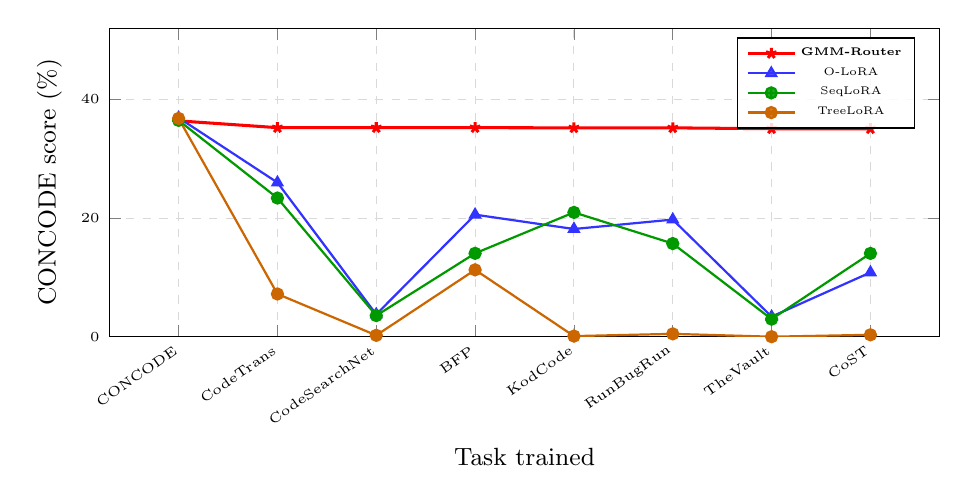
\begin{tikzpicture}
\begin{axis}[
    width=\linewidth, height=5.5cm,
    xlabel={Task trained},
    ylabel={CONCODE score (\%)},
    xtick={0,1,2,3,4,5,6,7},
    xticklabels={CONCODE,CodeTrans,CodeSearchNet,BFP,KodCode,RunBugRun,TheVault,CoST},
    xticklabel style={rotate=35, anchor=east, font=\tiny, yshift=-3pt},
    ymin=0, ymax=52,
    grid=major,
    grid style={dashed, gray!30},
    legend pos=north east,
    legend style={font=\tiny, nodes={scale=0.8}, draw=black, fill=white, fill opacity=0.85, text opacity=1},
    tick label style={font=\tiny},
    label style={font=\small},
]
\addplot[color=red, mark=star, thick, line width=1.1pt]
    coordinates {(0,36.39)(1,35.24)(2,35.24)(3,35.24)(4,35.21)(5,35.21)(6,35.06)(7,35.06)};
\addlegendentry{\textbf{GMM-Router}}
\addplot[color=blue!80, mark=triangle*, thick]
    coordinates {(0,36.91)(1,25.99)(2,3.77)(3,20.58)(4,18.16)(5,19.75)(6,3.39)(7,10.84)};
\addlegendentry{O-LoRA}
\addplot[color=green!60!black, mark=oplus*, thick]
    coordinates {(0,36.47)(1,23.38)(2,3.57)(3,14.06)(4,20.96)(5,15.71)(6,2.97)(7,14.05)};
\addlegendentry{SeqLoRA}
\addplot[color=orange!80!black, mark=otimes*, thick]
    coordinates {(0,36.80)(1,7.21)(2,0.24)(3,11.28)(4,0.11)(5,0.49)(6,0.01)(7,0.33)};
\addlegendentry{TreeLoRA}
\end{axis}
\end{tikzpicture}
\caption{Retained CONCODE score after each task in the CodeTask sequence. GMM-Router remains nearly flat ($36.39\%\to35.06\%$); O-LoRA and SeqLoRA show severe drops with partial recovery; TreeLoRA suffers substantial catastrophic forgetting.}
\label{fig:forgetting_concode}
\end{figure}

\paragraph{Executable benchmark.} Table~\ref{tab:bwt_exec} shows a different pattern. GMM-Router and O-LoRA show negative BWT on both Pass@1 and Pass@5, indicating net forgetting, because the instruction router's GMM boundaries shift as later language experts are added, and this drift is more pronounced here than on CodeTask since all nine languages share deep syntactic overlap, so their GMM regions sit close together and a new language's GMM displaces boundaries more than in the type-diverse CodeTask sequence. SeqLoRA and TreeLoRA instead show positive BWT, benefiting directly from cross-language reinforcement in their shared parameters. On FM, GMM-Router is competitive on Pass@1 ($1.77\%$, versus O-LoRA's $1.62\%$) and lowest on Pass@5 ($3.83\%$): because each adapter is frozen after training, no single later step can catastrophically overwrite it, so forgetting accumulates gradually through routing drift rather than through parameter overwriting, keeping worst-case single-step drops small; SeqLoRA and TreeLoRA show the opposite trade-off, with positive BWT but much higher FM ($6.92\%$ and $6.38\%$ Pass@1). All four methods show large FWT, and GMM-Router leads on Pass@5 FWT ($+25.97\%$) because each language adapter trains exclusively on its own data without competing gradients from other languages in a shared parameter space, fitting the target distribution more tightly than shared-parameter methods must. Swift illustrates the isolation guarantee directly: GMM-Router's retained Swift Pass@1 starts and ends the remaining eight-task sequence at exactly $66.40\%$ (dipping to $63.20\%$ at one intermediate step before returning), whereas TreeLoRA erodes by $2.4$pp and O-LoRA/SeqLoRA start lower but rise through cross-language reinforcement.

\begin{table}[t]
\centering
\caption{BWT, FM, and FWT (\%) on the executable benchmark. Positive BWT indicates backward enhancement; lower FM is better; higher FWT indicates stronger in-task learning.}
\label{tab:bwt_exec}
\scriptsize
\resizebox{\linewidth}{!}{%
\begin{tabular}{lcccccc}
\toprule
\multirow{2}{*}{Method} & \multicolumn{2}{c}{BWT $\uparrow$} & \multicolumn{2}{c}{FM $\downarrow$} & \multicolumn{2}{c}{FWT $\uparrow$} \\
\cmidrule(lr){2-3}\cmidrule(lr){4-5}\cmidrule(lr){6-7}
 & P@1 (\%) & P@5 (\%) & P@1 (\%) & P@5 (\%) & P@1 (\%) & P@5 (\%) \\
\midrule
\textbf{GMM-Router} & $-1.22$ & $-2.61$ & $1.77$ & $3.83$ & $+20.94$ & $+25.97$ \\
O-LoRA     & $-0.59$ & $-1.36$ & $1.62$ & $4.51$ & $+19.61$ & $+18.85$ \\
SeqLoRA    & $+0.88$ & $+0.28$ & $6.92$ & $10.47$ & $+22.07$ & $+20.99$ \\
TreeLoRA   & $+1.67$ & $+3.68$ & $6.38$ & $8.44$ & $+21.08$ & $+18.63$ \\
\bottomrule
\end{tabular}%
}
\end{table}

Taken together, RQ3 shows a clear cross-benchmark contrast: on the diverse CodeTask sequence, per-expert isolation reduces net forgetting by more than an order of magnitude relative to the best shared-parameter baseline; on the homogeneous executable benchmark, routing drift from closely packed language GMMs causes mild net forgetting, but GMM-Router still keeps FM competitive and leads on Pass@5 FWT.

\subsection{RQ4: Iterative refinement}
\label{sec:refinement}

GMM-Router's Round-2 pipeline (Section~\ref{sec:traceback}) triggers only for samples where all five Round-1 candidates fail. Table~\ref{tab:ablation_refinement} ablates its two components: the traceback router with JSD-gated combination, and an optional adapter-refinement step.

\begin{table}[t]
\centering
\caption{Ablation of Round-2 pipeline components on the executable benchmark. Best averages in bold.}
\label{tab:ablation_refinement}
\small
\resizebox{\linewidth}{!}{%
\begin{tabular}{lcc}
\toprule
Configuration & Avg.\ Pass@1 (\%) & Avg.\ Pass@5 (\%) \\
\midrule
Round-1 only & 33.04 & 41.66 \\
Round-2, original adapter + JSD & \textbf{34.40} & \textbf{47.75} \\
Round-2, refined adapter + JSD & 33.62 & 43.97 \\
\bottomrule
\end{tabular}%
}
\end{table}

Adding Round-2 with the original adapter and JSD-gated combination raises average Pass@1 by $1.36$pp ($33.04\%\to34.40\%$) and Pass@5 by $6.09$ points ($41.66\%\to47.75\%$), concentrated on Rust ($+9.05\%$ Pass@1, $+39.62\%$ Pass@5) and Java ($+2.65\%$ Pass@1, $+13.18\%$ Pass@5), the two languages where Round-1 candidates most often exhaust all five attempts. Table~\ref{tab:r2_lang} breaks Round-2 coverage (fraction of samples triggering Round-2) and lift (fraction of triggered samples recovered) down by language at the final training step.

\begin{table}[t]
\centering
\caption{Round-2 coverage and lift per language at the final training step. Languages sorted by lift, descending.}
\label{tab:r2_lang}
\small
\begin{tabular}{lrrr}
\toprule
Language   & Coverage (\%) & Triggered/Total & Lift (\%) \\
\midrule
Rust       & 81.1 & 43/53 & 48.8 \\
Java       & 67.9 & 36/53 & 19.4 \\
Shell      & 64.0 & 32/50 &  3.1 \\
C++        & 92.0 & 46/50 &  0.0 \\
C\#        & 92.0 & 46/50 &  0.0 \\
Python     & 54.0 & 27/50 &  0.0 \\
PHP        & 54.0 & 27/50 &  0.0 \\
Swift      & 20.0 & 10/50 &  0.0 \\
TypeScript &  0.0 &  0/50 & --- \\
\bottomrule
\end{tabular}
\end{table}

C++ and C\# both trigger Round-2 on 92\% of their test samples yet achieve zero lift: their failures stem from generation quality rather than routing mismatch, so redirecting to a different expert does not help. TypeScript never triggers Round-2 because every Round-1 candidate already passes, consistent with its near-perfect Table~\ref{tab:exec_p1}/\ref{tab:exec_p5} scores. Refining each adapter on error-repair pairs (Table~\ref{tab:ablation_refinement}, third row) gives a mixed picture: Java Pass@5 rises further (to $47.17\%$), but Rust declines markedly ($58.49\%\to24.53\%$ Pass@5), likely because repair targets are drawn from any passing candidate rather than one that specifically addresses the traceback shown, so the refined adapter can be trained on a repair signal that is not causally linked to the reported error (Section~\ref{sec:limitations}).

Table~\ref{tab:jsd_summary} isolates the Round-2 routing rule itself, holding the original (non-refined) adapters fixed and comparing traceback-alone routing, an unweighted sum of instruction and traceback log-posteriors, and the JSD-gated combination of Eq.~\eqref{eq:jsd_gated}.

\begin{table}[t]
\centering
\caption{Average Pass@1/Pass@5 (\%) under four Round-2 routing strategies (original adapters).}
\label{tab:jsd_summary}
\small
\begin{tabular}{lcc}
\toprule
Configuration & Avg.\ Pass@1 (\%) & Avg.\ Pass@5 (\%) \\
\midrule
Round-1 only               & 33.04 & 41.66 \\
Traceback alone            & 34.13 & 46.48 \\
Unweighted sum              & 34.13 & 46.48 \\
\textbf{JSD-gated}          & \textbf{34.40} & \textbf{47.75} \\
\bottomrule
\end{tabular}
\end{table}

Traceback routing is the primary driver of Round-2 gains: moving from Round-1 to any Round-2 variant, Rust improves most (Pass@1 $10.57\%\to19.62\%$, Pass@5 $18.87\%\to58.49\%$), since Rust's distinctive borrow-checker and lifetime diagnostics let the traceback GMM identify and redirect these failures regardless of how the instruction router scored the problem; six of the nine languages show no change across Round-2 variants because their Round-1 candidates either already pass (TypeScript) or fail in ways rerouting cannot fix (C++, C\#, Python, PHP, Swift). The unweighted sum produces results identical to traceback alone across all languages, because on samples that already exhausted five Round-1 attempts the traceback GMM assigns much sharper posterior mass to a single expert than the instruction GMM does, so summing the two log-posteriors does not change the top-ranked expert. JSD gating is what recovers the remaining conflicted samples: it behaves like the combined posterior when the two routers agree and blends toward uniform when they conflict, which prevents overconfident misrouting and lifts Java (Pass@5 $35.85\%\to45.28\%$, $+9.43$pp; Pass@1 $+1.89$pp) and Shell (Pass@5 $+2$pp) beyond what traceback-alone or the unweighted sum achieve; Rust is unaffected because the traceback router alone already accounts for most of its gain.

\subsection{Discussion}
\label{sec:discussion}

\subsubsection{Cross-benchmark comparison}
\label{sec:crossbench}

Figure~\ref{fig:method_comparison} plots each method's CodeTask average against its executable Pass@1, exposing a tension among the baselines: methods that maximize executable Pass@1 through parameter or gradient sharing (SeqLoRA, TreeLoRA) forget on the diverse CodeTask sequence, while methods that isolate tasks to protect CodeTask performance (O-LoRA, Online-CL-LLM) lack a dedicated task-agnostic routing mechanism and only reach moderate executable Pass@1. GMM-Router occupies a distinct position: $51.62\%$ on CodeTask --- $8.85$pp above O-LoRA and $16.72$pp above SeqLoRA --- while its $34.40\%$ executable Pass@1 exceeds the non-iterative upper bound, and its $47.75\%$ Pass@5 leads all methods. This is consistent with per-task expert isolation and soft distribution-level routing being complementary: isolation prevents forgetting on diverse sequences, while soft routing and iterative refinement provide candidate diversity and recovery on homogeneous ones.

\begin{figure}[t]
\centering
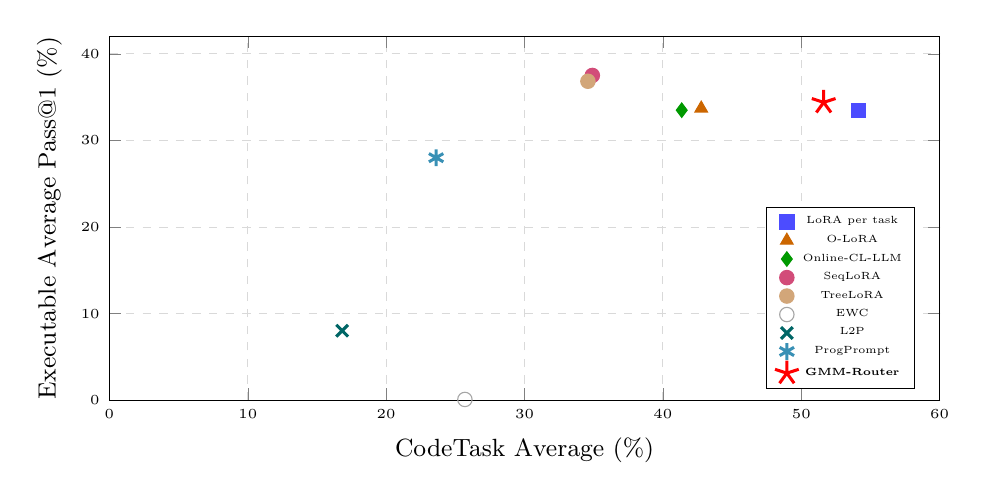
\begin{tikzpicture}
\begin{axis}[
    width=\linewidth, height=6.2cm,
    xlabel={CodeTask Average (\%)},
    ylabel={Executable Average Pass@1 (\%)},
    xmin=0, xmax=60,
    ymin=0, ymax=42,
    grid=major,
    grid style={dashed, gray!30},
    legend pos=south east,
    legend style={font=\tiny, nodes={scale=0.75}, draw=black},
    tick label style={font=\tiny},
    label style={font=\small},
]
\addplot[only marks, mark=square*, mark size=2.6pt, color=blue!70]
    coordinates {(54.15, 33.46)};
\addlegendentry{LoRA per task}
\addplot[only marks, mark=triangle*, mark size=2.6pt, color=orange!80!black]
    coordinates {(42.77, 33.71)};
\addlegendentry{O-LoRA}
\addplot[only marks, mark=diamond*, mark size=2.6pt, color=green!60!black]
    coordinates {(41.36, 33.50)};
\addlegendentry{Online-CL-LLM}
\addplot[only marks, mark=oplus*, mark size=2.6pt, color=purple!70]
    coordinates {(34.90, 37.51)};
\addlegendentry{SeqLoRA}
\addplot[only marks, mark=otimes*, mark size=2.6pt, color=brown!70]
    coordinates {(34.58, 36.84)};
\addlegendentry{TreeLoRA}
\addplot[only marks, mark=o, mark size=2.6pt, color=gray!70]
    coordinates {(25.69, 0.09)};
\addlegendentry{EWC}
\addplot[only marks, mark=x, mark size=3pt, color=teal!80!black, line width=1.1pt]
    coordinates {(16.82, 8.03)};
\addlegendentry{L2P}
\addplot[only marks, mark=asterisk, mark size=3pt, color=cyan!70!black, line width=1.1pt]
    coordinates {(23.61, 28.01)};
\addlegendentry{ProgPrompt}
\addplot[only marks, mark=star, mark size=4.5pt, color=red, line width=1.1pt]
    coordinates {(51.62, 34.40)};
\addlegendentry{\textbf{GMM-Router}}
\end{axis}
\end{tikzpicture}
\caption{CodeTask average (\%) vs.\ executable average Pass@1 (\%) for each method. LoRA per task is the upper bound. Methods in the upper-right corner are preferred; methods that trade one benchmark for the other appear off-diagonal.}
\label{fig:method_comparison}
\end{figure}

\subsubsection{Qualitative example: Round-2 recovery via traceback routing}
\label{sec:error_analysis}

The following case illustrates why the traceback router recovers samples the instruction router cannot. For a Rust task (implementing \texttt{is\_arithmetic\_sequence}), the instruction router assigns $\alpha_{\text{cpp}}=1.0$ with zero weight elsewhere, and all five Round-1 candidates fail to compile with \texttt{error[E0601]: `main` function not found}: the C++-trained adapter generates a bare function body following the C++ submission convention, where the harness supplies its own entry point, but Rust requires an explicit \texttt{fn main()} to compile as a standalone binary regardless of whether the function logic is correct. In Round-2, the traceback GMM redistributes routing weight to $\alpha_{\text{rust}}=0.384$ (Figure~\ref{fig:case_routing}), because \texttt{error[E0601]} is a diagnostic vocabulary specific to Rust's compilation model and absent from C++ output. The regenerated candidate is functionally identical to the Round-1 output except for the addition of \texttt{fn main()}, which the Rust adapter produces because its training data includes the standalone-binary scaffold. This example is representative of the pattern behind Table~\ref{tab:r2_lang}: the instruction GMM fails when generic problem phrasing makes two languages indistinguishable at the embedding level, while the traceback GMM succeeds because compilation errors are intrinsically language-specific diagnostics.

\begin{figure}[t]
\centering
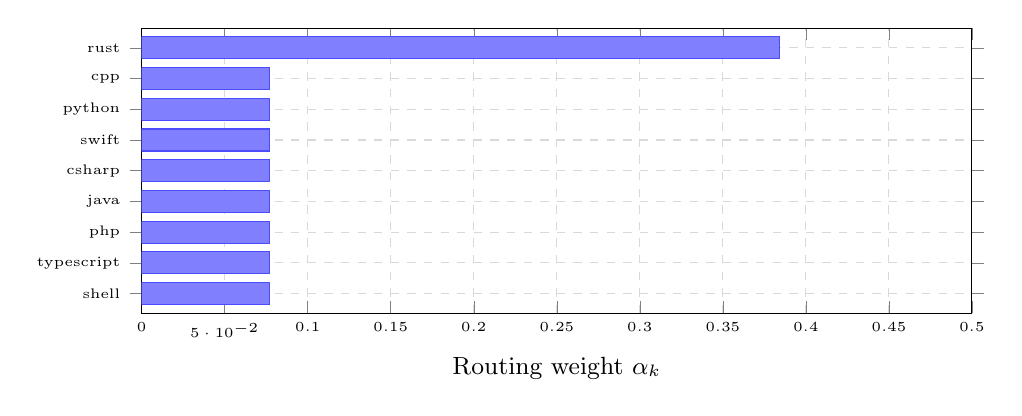
\begin{tikzpicture}
\begin{axis}[
    xbar, bar width=0.28cm,
    width=\linewidth, height=5.2cm,
    symbolic y coords={shell,typescript,php,java,csharp,swift,python,cpp,rust},
    ytick=data,
    xlabel={Routing weight $\alpha_k$},
    xmin=0, xmax=0.5,
    grid=major,
    grid style={dashed, gray!30},
    tick label style={font=\tiny},
    label style={font=\small},
    enlarge y limits=0.08,
]
\addplot[fill=blue!50, draw=blue!70]
    coordinates {
        (0.3839,rust) (0.0770,cpp)   (0.0770,python)
        (0.0770,swift) (0.0770,csharp) (0.0770,java)
        (0.0770,php)  (0.0770,typescript) (0.0770,shell)
    };
\end{axis}
\end{tikzpicture}
\caption{Round-2 routing weights $\alpha_k$ after traceback-GMM redistribution for the example in Section~\ref{sec:error_analysis}. The Rust expert rises from $0$ to $0.384$; the remaining weight spreads approximately evenly across the other eight experts.}
\label{fig:case_routing}
\end{figure}

\subsubsection{Limitations and threats to validity}
\label{sec:limitations}

\textbf{Construct validity.} BLEU and CodeBLEU, used on the CodeTask benchmark, cannot fully distinguish functionally correct code from code that merely resembles a reference (Section~\ref{sec:metrics}); this is mitigated by the executable benchmark's unit-test grading, but the two tracks are not directly comparable and are reported separately throughout.

\textbf{Internal validity.} All continual learning metrics (Eqs.~\eqref{eq:fm}--\eqref{eq:bwt_fwt}) depend on the fixed task order used during training (Section~\ref{sec:hyperparams}); a different order could change which tasks interfere with which, particularly on the executable benchmark where routing drift is order-dependent (Section~\ref{sec:forgetting}). The repair pairs used for adapter refinement (Section~\ref{sec:traceback}) pair a failed candidate's traceback with any passing candidate rather than one verified to resolve that specific error, which is a plausible explanation for the Rust regression in Table~\ref{tab:ablation_refinement} and is a limitation of the training signal rather than of the routing mechanism itself.

\textbf{External validity.} Experiments use a single 1.5B-parameter backbone (Section~\ref{sec:baselines}); routing behavior --- particularly the C++ attractor effect in Figure~\ref{fig:confusion_exec} --- may differ for backbones with different pretraining data or scale. The executable benchmark's test set is drawn from McEval and capped at 50--53 problems per language (Table~\ref{tab:exec_stats}), which bounds the precision of the per-language Pass@$k$ estimates in Tables~\ref{tab:exec_p1}--\ref{tab:exec_p5}.

\textbf{Conclusion validity.} Per-task expert isolation, while effective at preventing forgetting, limits transfer between related tasks; this is most visible on C\# and Rust in the executable benchmark (Section~\ref{sec:perlang}), where shared-adaptation baselines benefit from cross-language transfer that GMM-Router cannot replicate without an explicit sharing mechanism. Routing quality also depends on how well the frozen backbone separates task distributions at the chosen layer $\ell^*$; tasks with similar surface-level inputs but different output objectives, such as the nine syntactically related programming languages, are intrinsically harder to separate by density estimation alone (Section~\ref{sec:routing_analysis}). Finally, adapter storage grows linearly with the number of tasks, which may become a practical constraint on much longer task sequences than the eight- and nine-task streams studied here.
